\documentclass[a4paper]{article}

\usepackage[english, portuguese]{babel}
\usepackage[utf8x]{inputenc}
\usepackage[T1]{fontenc}

\usepackage[a4paper,top=3cm,bottom=2cm,left=3cm,right=3cm,marginparwidth=1.75cm]{geometry}

%% Useful packages
\usepackage{amsmath}
\usepackage{graphicx}
\usepackage[colorinlistoftodos]{todonotes}
\usepackage[colorlinks=true, allcolors=blue]{hyperref}

\usepackage{float} % Usado para posicionar imagens
\usepackage{enumitem} % Usado para criar listas enumeradas com letras
\usepackage{booktabs} % Usado para criar tabelas

\usepackage{listings}
\usepackage{color}
\usepackage{xcolor}

\definecolor{vgreen}{RGB}{104,180,104}
\definecolor{vblue}{RGB}{49,49,255}
\definecolor{vorange}{RGB}{255,143,102}

\lstdefinestyle{verilog-style}
{
    language=Verilog,
    basicstyle=\small\ttfamily,
    keywordstyle=\color{vblue},
    identifierstyle=\color{black},
    commentstyle=\color{vgreen},
    numbers=left,
    numberstyle=\tiny\color{black},
    numbersep=10pt,
    tabsize=4,
    showstringspaces = false,
    moredelim=*[s][\colorIndex]{[}{]},
    literate=*{:}{:}1
}

\lstdefinestyle{verilog-style-nolinenumber}
{
    language=Verilog,
    basicstyle=\small\ttfamily,
    keywordstyle=\color{vblue},
    identifierstyle=\color{black},
    commentstyle=\color{vgreen},
    numbers=none,
    numberstyle=\tiny\color{black},
    numbersep=10pt,
    tabsize=4,
    showstringspaces = false,
    moredelim=*[s][\colorIndex]{[}{]},
    literate=*{:}{:}1
}

\makeatletter
\newcommand*\@lbracket{[}
\newcommand*\@rbracket{]}
\newcommand*\@colon{:}
\newcommand*\colorIndex{%
    \edef\@temp{\the\lst@token}%
    \ifx\@temp\@lbracket \color{black}%
    \else\ifx\@temp\@rbracket \color{black}%
    \else\ifx\@temp\@colon \color{black}%
    \else \color{vorange}%
    \fi\fi\fi
}
\makeatother

\usepackage{trace}


\title{Curso de Verilog - Dia 1}
\author{Caio Rodrigo, Jorge Reis}
\date{} % No Date
%%%%%%%%%%%%%%%%%%%%%%%%%%%%%%%%%%%%%%%%%%%%%%%%%%%%%%%%%%%%%%%%%
%***** Document *****%
\begin{document}
\maketitle

%***** Prática 0 *****%
\section*{Prática 0 - Hello World}

Vamos agora realizar um de exemplo Hello World em Verilog para se habituar com o Vivado e aprender a executar arquivos em Verilog.

\subsection*{Criando o Projeto}

\begin{enumerate}
\item Crie um projeto no Vivado;
\item \textbf{Project Name}: escolha um  nome e o local do projeto;
\item \textbf{Project Type}: marque "RTL Project" e "Do not specify sources at this time";
\item \textbf{Default Part}: aqui é possível escolher a FPGA para a síntese. Como nenhuma síntese será feita, a escolha é irrelevante;
\item Finish. 
\end{enumerate}

\subsection*{Adicionando Arquivos}
O Vivado abrirá o projeto e agora é preciso criar o arquivo do código fonte. Para isso, clique em no símbolo do "+". Para as práticas 0 e 1 será preciso criar arquivos de \textbf{simulação} e para a prática 2 será preciso criar arquivos de \textbf{design}.

\begin{figure}[ht]
\centering
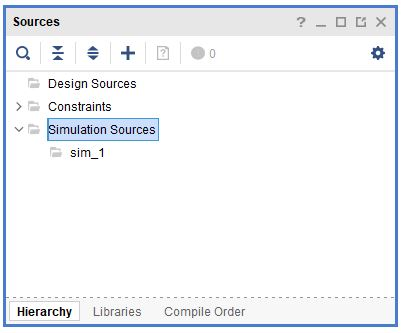
\includegraphics[width=0.3\textwidth]{images/addfile.jpg}
\end{figure}

Na janela que se abriu, siga o seguintes passos:

\begin{enumerate}
\item Selecione "Add or create simulation sources";
\item Clique em "Create File", digite o nome do arquivo a ser criado e deixa o "File Type" como Verilog;
\item \textbf{Define Module} aqui é possível criar entradas e saídas para o módulo do arquivo criado. Isso não será necessário para o exemplo;
\item O arquivo foi criado dentro da pasta "Simulation Sources".
\end{enumerate}

Abra o arquivo, por padrão, o Vivado gera um módulo já com timescale, um header e o protótipo do módulo. Acrescente ao código gerado a diretiva \textbf{Initial} do Verilog, conforme o código abaixo:

\begin{figure}[H]
\centering
	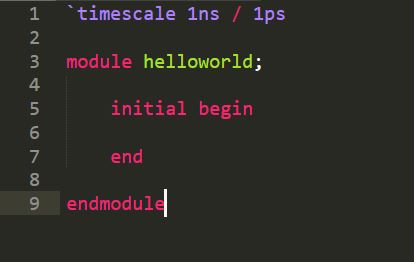
\includegraphics[width=0.3\textwidth]{images/helloworld.jpg}
\end{figure}

O initial é importante para a execução de \textbf{System Tasks} e possibilita a atribuição de variáveis como será visto mais adiante no curso. Agora é possível utilizar a \textbf{System Task \$display} para fazer o \textbf{Hello World}. 

\subsection*{Executando Arquivos}

A única forma de "executar" arquivos em Verilog é por meio de simulação. Para isso, clique em \textbf{Simulation} > \textbf{Run Simulation} > \textbf{Run Behavioral Simulation} em \textbf{Flow Navigator}, localizado no lado esquerdo do Vivado.

Se tudo tiver ocorrido corretamente, a mensagem será exibida na janela \textbf{Tcl Console} localizada na parte inferior do programa.

%***** Prática 1 - Trabalhando com Números *****%
\section*{Prática 1 - Trabalhando com Números}

\subsection*{System Task \$display}

A system task \$display serve para imprimir textos no terminal do simulador. Ela tem seu funcionamento similar à função \textbf{printf} da linguagem C.
\begin{lstlisting}[style={verilog-style-nolinenumber}]
$display("Ola"); // Printa "Ola" no terminal
\end{lstlisting}

O print do valor de uma variável é possível por meio do caractere "\%" da seguinte forma:
\begin{lstlisting}[style={verilog-style-nolinenumber}]
$display("%d", var); // Printa a variavel "var" em decimal "%d"
$display("%d e %b", var1, var2); // Printa a variavel "var1" em decimal
								 // e "var2" em binario
\end{lstlisting}

Caso queira utilizar o caractere "\%", use ele duas vezes na string do display: "\%\%".


% Please add the following required packages to your document preamble:

\begin{table}[H]
\caption{Especificação dos formatos de strings}
\begin{tabular}{@{}ll@{}}
\toprule
\multicolumn{1}{c}{Format} & \multicolumn{1}{c}{Display}                                             \\ \midrule
\%d ou \%D                 & Mostra a variável em decimal                                            \\
\%b ou \%B                 & Mostra a variável em binário                                            \\
\%s ou \%S                 & Mostra a string                                                         \\
\%h ou \%H                 & Mostra a variável em hexadecimal                                        \\
\%c ou \%C                 & Mostra um caractere ASCII                                               \\
\%m ou \%M                 & Mostra o nome hierárquico do módulo (não precisa de argumento)          \\
\%v ou \%V                 & Mostra a força do sinal                                                 \\
\%o ou \%O                 & Mostra a variável em octal                                              \\
\%t ou \%T                 & Mostra o tempo de simulação                                             \\
\%e ou \%E                 & Mostra um número real em notação científica (EX: 3e10)                  \\
\%f ou \%F                 & Mostra um número real em formato decimal (EX: 2.13)                     \\
\%g ou \%G                 & Mostra um número real em notação científica ou decimal, o que for menor \\ \bottomrule
\end{tabular}
\end{table}

%% New Page %%
\newpage
%%%%%%%%%%%%%%

\subsection*{Atividades}
Utilizando a simulação e a task \textbf{\$display}, faça as atividades abaixo e confira os resultados no Tcl Console.

\begin{enumerate}
\item Escreva os seguintes números:
		\begin{enumerate}
	  	\item Número decimal "123" como um número sized 8-bits
	  	\item Hexadecimal de 16-bits de valor desconhecido (tudo X)
        \item Número de 4-bits '-2' em hexadecimal. Compare com '-2' escrito na forma de complemento de dois em um registrador de 4 bits
       	\item Número hexadecimal unsized "1234"
		\end{enumerate}
\item Crie variáveis dos tipos V1 e V2, salve os números e compare-os utilizando a task display com os formatos abaixo.
        \begin{enumerate}
        \item V1 = (integer) 5; V2 = (reg[4:0]) 5; \%d e \%b
        \item V1 = (integer) -5; V2 = (reg[4:0]) -5; V3 = (reg signed[4:0]) -5; \%d e \%b
        \item V1 = (reg[4:0]) 3; V2 = (reg[0:4]) 3; \%b e \%b de V1[4] e V2[4]
        \item V1 = (integer) 3; V2 = (real) 3.0; \%d e \%b
        \end{enumerate}
	  	
\end{enumerate}

%****** Prática 2 - Gate Modelling
\section*{Prática 2 - Gate Modelling}

A modelagem no nível de abstração de gates se aproxima bastante com o que é feito em Eletrônica Digital. O desenvolvedor se preocupa em instanciar gates e conectá-los para criar o circuito desejado. Alguns exemplos de instanciações:
\begin{lstlisting}[style={verilog-style-nolinenumber}]
and a1 (out,in1,in2);		// Instanciacao basica
or or1 (out,in1,in2,in3);	// O numero de entradas pode ser maior que 2
not (out, in);				// Nao e preciso colocar o nome do gate para intancia-lo
// Repare que a primeira porta e sempre um output
\end{lstlisting}

Alguns gates que podem ser instanciados:  and, nand, or, nor, xor, xnor...

\subsection*{Atividades}
Utilize modelagem em nível de gates para criar os circuitos abaixo. Lembre-se de criar os arquivos como \textbf{design source} e não \textbf{simulation source}

\begin{enumerate}
\item Multiplexador 2x1:
	\begin{figure}[H]
	\centering
	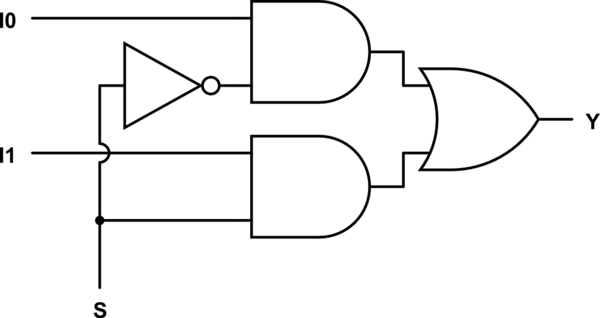
\includegraphics[width=0.3\textwidth]{images/mux2x1.jpg}
	\end{figure}
		
\item Full Adder:
	\begin{figure}[!h]
	\centering
	
\includegraphics[width=0.3\textwidth]{images/fulladder.jpg}
	\end{figure}
	
\end{enumerate}

\end{document}